\chapter{Interventional Radiology and Cardiac Catheterization}
\label{ch:interventional_radiology_cardiac_catheterization}

% Chapter-opening illustrated modality infographic.
\begin{center}
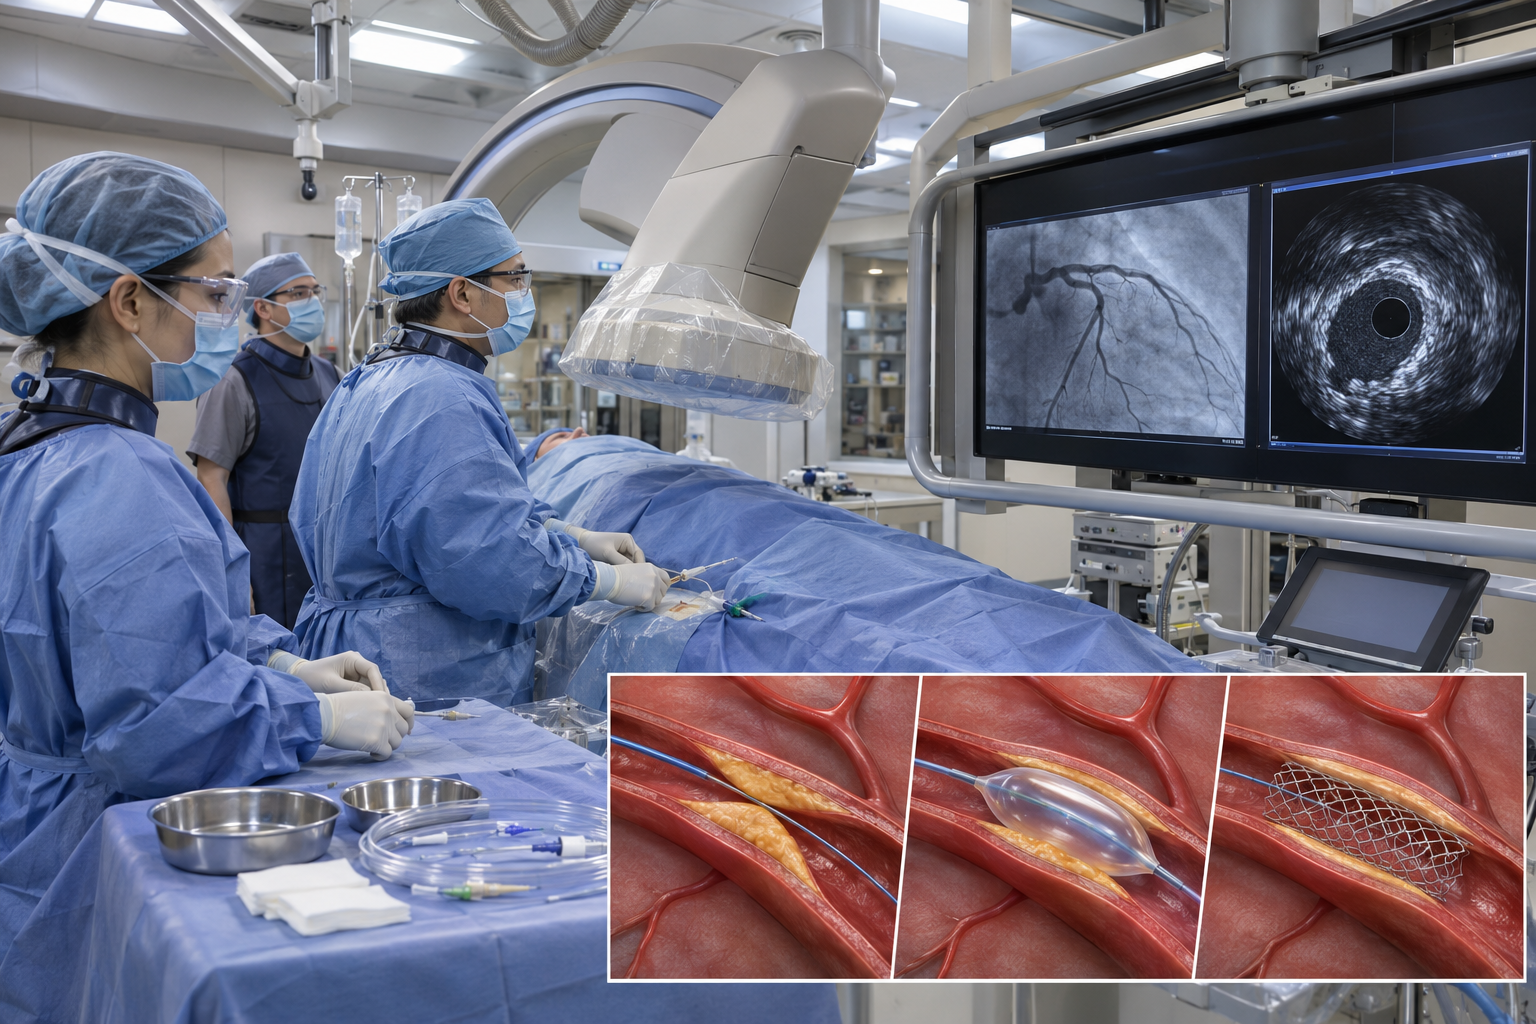
\includegraphics[width=\textwidth,keepaspectratio]{modalities/infographics/interventional_radiology_cardiac_cath_realistic.png}
\end{center}
\begin{center}\footnotesize Image-guided procedures use live imaging to navigate devices and assess treatment; the inset schematically shows catheter-based coronary intervention. AI-generated illustration; no actual procedure is depicted.\end{center}

\section{Overview}
Interventional radiology (IR) and cardiac catheterization are minimally invasive medical disciplines that use image guidance to perform diagnostic and therapeutic procedures. Unlike conventional diagnostic imaging, these disciplines enable physicians to interact directly with anatomical structures using catheters, guidewires, needles, balloons, stents, and other medical devices.

Imaging modalities employed include fluoroscopy, digital subtraction angiography (DSA), computed tomography (CT), ultrasound and Doppler ultrasound, cone-beam CT (CBCT), magnetic resonance imaging (MRI), intravascular ultrasound (IVUS), optical coherence tomography (OCT), and intracardiac echocardiography (ICE).

The catalogue includes diseases, characteristic imaging findings, and associated interventional procedures. It spans diagnostic findings, therapeutic indications, and specialized procedures. Some entries overlap; interventions may be appropriate only for selected patients or remain emerging applications. Individual indications require validation against current clinical guidelines.

\section{Where image-guided intervention is used}
The numbered entries below describe example imaging findings and related procedures. They are not treatment recommendations; decisions depend on the patient's condition, anatomy, risks, and current professional guidance.

\subsection{Part I: Interventional radiology}

\subsubsection{Peripheral arterial diseases}
\begin{enumerate}[leftmargin=*,itemsep=0.45em,topsep=0.4em]
\item \textbf{Acute limb ischemia.} Useful imaging findings include: Abrupt arterial contrast cutoff. Interventional Procedure: Thrombectomy, catheter-directed thrombolysis.
\item \textbf{Aortoiliac occlusive disease.} Useful imaging findings include: Aortoiliac stenosis or occlusion. Interventional Procedure: Angioplasty, stenting.
\item \textbf{Arterial dissection.} Useful imaging findings include: Intimal flap or false lumen. Interventional Procedure: Selected stent placement.
\item \textbf{Arterial embolism.} Useful imaging findings include: Abrupt intraluminal filling defect. Interventional Procedure: Catheter thrombectomy.
\item \textbf{Arterial thrombosis.} Useful imaging findings include: Intraluminal filling defect or complete occlusion. Interventional Procedure: Thrombectomy, thrombolysis.
\item \textbf{Buerger disease.} Useful imaging findings include: Distal arterial occlusions and corkscrew collaterals. Interventional Procedure: Selected endovascular revascularization.
\item \textbf{Chronic limb-threatening ischemia.} Useful imaging findings include: Multilevel occlusive disease and poor distal runoff. Interventional Procedure: Endovascular revascularization.
\item \textbf{Femoral artery stenosis.} Useful imaging findings include: Focal luminal narrowing. Interventional Procedure: Angioplasty, stenting.
\item \textbf{Leriche syndrome.} Useful imaging findings include: Distal aortic and iliac artery occlusion. Interventional Procedure: Endovascular revascularization.
\item \textbf{Peripheral arterial disease.} Useful imaging findings include: Arterial narrowing and impaired distal contrast flow. Interventional Procedure: Angioplasty, stenting.
\item \textbf{Popliteal artery stenosis.} Useful imaging findings include: Narrowing of the popliteal artery. Interventional Procedure: Angioplasty.
\item \textbf{Subclavian artery stenosis.} Useful imaging findings include: Focal proximal arterial narrowing. Interventional Procedure: Angioplasty, stenting.
\item \textbf{Subclavian steal syndrome.} Useful imaging findings include: Reversal of vertebral arterial flow. Interventional Procedure: Subclavian artery stenting.
\item \textbf{Tibial artery occlusion.} Useful imaging findings include: Interrupted distal arterial flow. Interventional Procedure: Balloon angioplasty.
\item \textbf{Traumatic arterial injury.} Useful imaging findings include: Contrast extravasation, occlusion or pseudoaneurysm. Interventional Procedure: Embolization, covered stent.
\end{enumerate}

\subsubsection{Aortic and visceral arterial diseases}
\begin{enumerate}[leftmargin=*,itemsep=0.45em,topsep=0.4em]
\item \textbf{Abdominal aortic aneurysm.} Useful imaging findings include: Abnormal aortic dilatation. Interventional Procedure: EVAR.
\item \textbf{Acute mesenteric ischemia.} Useful imaging findings include: Mesenteric arterial occlusion. Interventional Procedure: Urgent revascularization; endovascular treatment in selected patients without peritonitis or suspected bowel necrosis.
\item \textbf{Chronic mesenteric ischemia.} Useful imaging findings include: Mesenteric arterial stenosis. Interventional Procedure: Angioplasty, stenting.
\item \textbf{Complicated type B aortic dissection.} Useful imaging findings include: True and false lumens, branch compromise. Interventional Procedure: TEVAR.
\item \textbf{Fibromuscular dysplasia.} Useful imaging findings include: Characteristic string-of-beads appearance. Interventional Procedure: Selected balloon angioplasty.
\item \textbf{Hepatic artery aneurysm.} Useful imaging findings include: Abnormal hepatic arterial dilatation. Interventional Procedure: Embolization, covered stent.
\item \textbf{Penetrating aortic ulcer.} Useful imaging findings include: Focal ulceration extending into the aortic wall. Interventional Procedure: Selected endovascular repair.
\item \textbf{Renal artery aneurysm.} Useful imaging findings include: Focal arterial dilatation. Interventional Procedure: Embolization, covered stent.
\item \textbf{Renal artery stenosis.} Useful imaging findings include: Focal renal arterial narrowing. Interventional Procedure: Selected angioplasty or stenting.
\item \textbf{Splenic artery aneurysm.} Useful imaging findings include: Focal splenic arterial dilatation. Interventional Procedure: Coil embolization.
\item \textbf{Thoracic aortic aneurysm.} Useful imaging findings include: Thoracic aortic dilatation. Interventional Procedure: TEVAR.
\item \textbf{Traumatic aortic injury.} Useful imaging findings include: Aortic disruption or pseudoaneurysm. Interventional Procedure: TEVAR.
\item \textbf{Type I endoleak.} Useful imaging findings include: Contrast leakage at graft attachment site. Interventional Procedure: Endograft extension.
\item \textbf{Type II endoleak.} Useful imaging findings include: Retrograde filling of aneurysm sac. Interventional Procedure: Selected embolization.
\item \textbf{Type III endoleak.} Useful imaging findings include: Leakage through graft defect or component separation. Interventional Procedure: Endograft relining.
\item \textbf{Visceral artery pseudoaneurysm.} Useful imaging findings include: Contrast-filled sac communicating with an artery. Interventional Procedure: Embolization.
\end{enumerate}

\subsubsection{Neurological and cerebrovascular diseases}
\begin{enumerate}[leftmargin=*,itemsep=0.45em,topsep=0.4em]
\item \textbf{Acute large-vessel ischemic stroke.} Useful imaging findings include: Abrupt intracranial arterial occlusion. Interventional Procedure: Mechanical thrombectomy.
\item \textbf{Carotid-cavernous fistula.} Useful imaging findings include: Early cavernous sinus opacification. Interventional Procedure: Endovascular embolization.
\item \textbf{Cerebral arteriovenous malformation.} Useful imaging findings include: Abnormal vascular nidus and early venous drainage. Interventional Procedure: Selected embolization.
\item \textbf{Cerebral vasospasm.} Useful imaging findings include: Segmental intracranial arterial narrowing. Interventional Procedure: Intra-arterial vasodilators, angioplasty.
\item \textbf{Cerebral venous sinus thrombosis.} Useful imaging findings include: Venous filling defects. Interventional Procedure: Selected rescue thrombectomy.
\item \textbf{Chronic subdural hematoma.} Useful imaging findings include: Hematoma-associated meningeal vascular supply. Interventional Procedure: Middle meningeal artery embolization.
\item \textbf{Dural arteriovenous fistula.} Useful imaging findings include: Abnormal dural arterial-to-venous communication. Interventional Procedure: Transarterial or transvenous embolization.
\item \textbf{Fusiform cerebral aneurysm.} Useful imaging findings include: Segmental arterial dilatation. Interventional Procedure: Selected flow diversion.
\item \textbf{Idiopathic intracranial hypertension.} Useful imaging findings include: Venous sinus stenosis with pressure gradient. Interventional Procedure: Selected venous sinus stenting.
\item \textbf{Internal carotid artery stenosis.} Useful imaging findings include: Luminal narrowing. Interventional Procedure: Selected carotid artery stenting.
\item \textbf{Intracranial aneurysm.} Useful imaging findings include: Focal arterial outpouching. Interventional Procedure: Coil embolization, flow diversion.
\item \textbf{Intracranial arterial stenosis.} Useful imaging findings include: Focal intracranial vascular narrowing. Interventional Procedure: Selected angioplasty or stenting.
\item \textbf{Ruptured cerebral aneurysm.} Useful imaging findings include: Aneurysmal lesion associated with hemorrhage. Interventional Procedure: Endovascular coiling.
\item \textbf{Spinal arteriovenous malformation.} Useful imaging findings include: Abnormal spinal vascular network. Interventional Procedure: Selected embolization.
\item \textbf{Spinal dural arteriovenous fistula.} Useful imaging findings include: Abnormal spinal venous drainage. Interventional Procedure: Selected embolization.
\end{enumerate}

\subsubsection{Venous and thromboembolic diseases}
\begin{enumerate}[leftmargin=*,itemsep=0.45em,topsep=0.4em]
\item \textbf{Central venous stenosis.} Useful imaging findings include: Narrowing with collateral venous drainage. Interventional Procedure: Venoplasty.
\item \textbf{Chronic venous obstruction.} Useful imaging findings include: Occlusion and collateral formation. Interventional Procedure: Venous recanalization, stenting.
\item \textbf{Deep vein thrombosis.} Useful imaging findings include: Venous filling defect or absent flow. Interventional Procedure: Selected thrombectomy or thrombolysis.
\item \textbf{High-risk pulmonary embolism.} Useful imaging findings include: Extensive arterial obstruction and impaired perfusion. Interventional Procedure: Catheter thrombectomy or thrombolysis in selected patients.
\item \textbf{Iliofemoral venous thrombosis.} Useful imaging findings include: Extensive proximal venous occlusion. Interventional Procedure: Selected catheter thrombectomy.
\item \textbf{Inferior vena cava filter thrombosis.} Useful imaging findings include: Thrombus involving implanted filter. Interventional Procedure: Selected thrombectomy.
\item \textbf{Inferior vena cava obstruction.} Useful imaging findings include: Caval narrowing or occlusion. Interventional Procedure: Venoplasty, stenting.
\item \textbf{May--Thurner syndrome.} Useful imaging findings include: Left iliac vein compression. Interventional Procedure: Stenting in selected patients with significant symptoms and confirmed outflow obstruction.
\item \textbf{Nutcracker syndrome.} Useful imaging findings include: Left renal vein compression. Interventional Procedure: Selected venous intervention.
\item \textbf{Pelvic venous disorder.} Useful imaging findings include: Dilated pelvic veins and pathological reflux. Interventional Procedure: Selected venous embolization.
\item \textbf{Pulmonary embolism.} Useful imaging findings include: Pulmonary arterial filling defects. Interventional Procedure: Selected catheter-directed therapy.
\item \textbf{Superior vena cava syndrome.} Useful imaging findings include: Central venous stenosis or obstruction. Interventional Procedure: Venous stenting.
\item \textbf{Varicocele.} Useful imaging findings include: Dilated pampiniform veins with reflux. Interventional Procedure: Gonadal vein embolization.
\item \textbf{Varicose veins.} Useful imaging findings include: Venous dilatation and reflux. Interventional Procedure: Endovenous ablation.
\item \textbf{Venous malformation.} Useful imaging findings include: Abnormal slow-flow vascular spaces. Interventional Procedure: Sclerotherapy.
\end{enumerate}

\subsubsection{Hemorrhagic conditions}
\begin{enumerate}[leftmargin=*,itemsep=0.45em,topsep=0.4em]
\item \textbf{Acute gastrointestinal hemorrhage.} Useful imaging findings include: Active contrast extravasation into bowel. Interventional Procedure: Transarterial embolization.
\item \textbf{Diverticular hemorrhage.} Useful imaging findings include: Focal colonic arterial extravasation. Interventional Procedure: Superselective embolization.
\item \textbf{Hemorrhagic renal angiomyolipoma.} Useful imaging findings include: Abnormal tumor vessels and aneurysms. Interventional Procedure: Selective arterial embolization.
\item \textbf{Massive hemoptysis.} Useful imaging findings include: Abnormal hypertrophied bronchial arteries. Interventional Procedure: Bronchial artery embolization.
\item \textbf{Peptic ulcer hemorrhage.} Useful imaging findings include: Bleeding gastroduodenal arterial branch. Interventional Procedure: Arterial embolization.
\item \textbf{Postoperative hemorrhage.} Useful imaging findings include: Active extravasation or pseudoaneurysm. Interventional Procedure: Selective embolization.
\item \textbf{Postpartum hemorrhage.} Useful imaging findings include: Abnormal uterine vascularity or extravasation. Interventional Procedure: Uterine artery embolization.
\item \textbf{Rectus sheath hematoma.} Useful imaging findings include: Bleeding epigastric arterial branch. Interventional Procedure: Arterial embolization.
\item \textbf{Refractory epistaxis.} Useful imaging findings include: Abnormal nasal arterial supply. Interventional Procedure: Selected arterial embolization.
\item \textbf{Renal hemorrhage.} Useful imaging findings include: Renal arterial extravasation. Interventional Procedure: Selective renal embolization.
\item \textbf{Retroperitoneal hemorrhage.} Useful imaging findings include: Active arterial extravasation. Interventional Procedure: Transarterial embolization.
\item \textbf{Traumatic hepatic hemorrhage.} Useful imaging findings include: Hepatic arterial extravasation. Interventional Procedure: Hepatic artery embolization.
\item \textbf{Traumatic pelvic hemorrhage.} Useful imaging findings include: Pelvic arterial contrast extravasation. Interventional Procedure: Pelvic arterial embolization.
\item \textbf{Traumatic splenic hemorrhage.} Useful imaging findings include: Splenic vascular injury or pseudoaneurysm. Interventional Procedure: Splenic artery embolization.
\item \textbf{Tumor-associated hemorrhage.} Useful imaging findings include: Abnormal tumor vascularity with bleeding. Interventional Procedure: Tumor embolization.
\end{enumerate}

\subsubsection{Hepatic and portal venous diseases}
\begin{enumerate}[leftmargin=*,itemsep=0.45em,topsep=0.4em]
\item \textbf{Budd--Chiari syndrome.} Useful imaging findings include: Hepatic venous outflow obstruction. Interventional Procedure: Angioplasty, stenting, TIPS.
\item \textbf{Congenital portosystemic shunt.} Useful imaging findings include: Abnormal portal-systemic communication. Interventional Procedure: Selected shunt embolization.
\item \textbf{Esophageal variceal hemorrhage.} Useful imaging findings include: Abnormal portosystemic collateral vessels. Interventional Procedure: TIPS for uncontrolled or recurrent bleeding, or early in selected high-risk patients.
\item \textbf{Gastric varices.} Useful imaging findings include: Dilated gastric collateral vessels. Interventional Procedure: BRTO, PARTO or TIPS.
\item \textbf{Hepatic abscess.} Useful imaging findings include: Fluid collection with inflammatory changes. Interventional Procedure: Percutaneous drainage.
\item \textbf{Hepatic artery stenosis after transplantation.} Useful imaging findings include: Focal arterial narrowing. Interventional Procedure: Selected angioplasty or stenting.
\item \textbf{Hepatic artery thrombosis.} Useful imaging findings include: Absent hepatic arterial flow. Interventional Procedure: Selected endovascular revascularization.
\item \textbf{Hepatic cyst.} Useful imaging findings include: Fluid-filled hepatic lesion. Interventional Procedure: Selected aspiration and sclerotherapy.
\item \textbf{Hepatic vein stenosis.} Useful imaging findings include: Impaired hepatic venous drainage. Interventional Procedure: Angioplasty, stenting.
\item \textbf{Portal hypertension.} Useful imaging findings include: Dilated portal vessels and collateral circulation. Interventional Procedure: TIPS in selected patients.
\item \textbf{Portal vein stenosis.} Useful imaging findings include: Focal luminal narrowing. Interventional Procedure: Angioplasty, stenting.
\item \textbf{Portal vein thrombosis.} Useful imaging findings include: Portal venous filling defect. Interventional Procedure: Selected recanalization.
\item \textbf{Refractory ascites.} Useful imaging findings include: Ascites associated with portal hypertension. Interventional Procedure: TIPS in selected patients after assessment of candidacy and alternatives.
\item \textbf{TIPS dysfunction.} Useful imaging findings include: Shunt stenosis or abnormal flow. Interventional Procedure: TIPS revision.
\end{enumerate}

\subsubsection{Hepatobiliary and pancreatic diseases}
\begin{enumerate}[leftmargin=*,itemsep=0.45em,topsep=0.4em]
\item \textbf{Acute cholecystitis in high-risk patients.} Useful imaging findings include: Gallbladder distension and inflammatory changes. Interventional Procedure: Percutaneous cholecystostomy.
\item \textbf{Benign biliary stricture.} Useful imaging findings include: Focal biliary narrowing. Interventional Procedure: Balloon dilatation, drainage.
\item \textbf{Biliary-enteric anastomotic stricture.} Useful imaging findings include: Narrowing at surgical anastomosis. Interventional Procedure: Balloon dilatation.
\item \textbf{Biloma.} Useful imaging findings include: Localized bile collection. Interventional Procedure: Percutaneous drainage.
\item \textbf{Cholangiocarcinoma.} Useful imaging findings include: Irregular malignant biliary obstruction. Interventional Procedure: Biliary drainage or stenting.
\item \textbf{Hilar biliary obstruction.} Useful imaging findings include: Obstruction at hepatic duct confluence. Interventional Procedure: Percutaneous biliary drainage.
\item \textbf{Infected pancreatic necrosis.} Useful imaging findings include: Complex necrotic collection. Interventional Procedure: Percutaneous drainage.
\item \textbf{Malignant biliary obstruction.} Useful imaging findings include: Biliary dilatation and obstructing lesion. Interventional Procedure: Percutaneous biliary drainage, stenting.
\item \textbf{Pancreatic abscess.} Useful imaging findings include: Localized infected collection. Interventional Procedure: Percutaneous drainage.
\item \textbf{Pancreatic pseudocyst.} Useful imaging findings include: Encapsulated pancreatic fluid collection. Interventional Procedure: Selected percutaneous drainage.
\item \textbf{Postoperative bile leak.} Useful imaging findings include: Extraluminal biliary contrast. Interventional Procedure: Biliary diversion, drainage.
\item \textbf{Retained biliary calculi.} Useful imaging findings include: Intraductal filling defects. Interventional Procedure: Selected percutaneous stone extraction.
\end{enumerate}

\subsubsection{Interventional oncology}
\begin{enumerate}[leftmargin=*,itemsep=0.45em,topsep=0.4em]
\item \textbf{Adrenal metastases.} Useful imaging findings include: Adrenal mass. Interventional Procedure: Selected thermal ablation.
\item \textbf{Colorectal liver metastases.} Useful imaging findings include: Focal hepatic metastatic lesions. Interventional Procedure: Selected ablation or radioembolization.
\item \textbf{Desmoid-type fibromatosis.} Useful imaging findings include: Infiltrative soft-tissue mass. Interventional Procedure: Selected cryoablation.
\item \textbf{Hepatocellular carcinoma.} Useful imaging findings include: Arterial hyperenhancement and possible washout. Interventional Procedure: TACE, TARE, thermal ablation.
\item \textbf{Hypervascular bone tumor.} Useful imaging findings include: Intense tumor vascularity. Interventional Procedure: Preoperative embolization.
\item \textbf{Intrahepatic cholangiocarcinoma.} Useful imaging findings include: Infiltrative or mass-forming hepatic tumor. Interventional Procedure: Selected radioembolization.
\item \textbf{Neuroendocrine liver metastases.} Useful imaging findings include: Hypervascular metastatic lesions. Interventional Procedure: Hepatic arterial embolization.
\item \textbf{Osteoid osteoma.} Useful imaging findings include: Small osseous nidus. Interventional Procedure: Radiofrequency ablation.
\item \textbf{Painful bone metastases.} Useful imaging findings include: Destructive or infiltrative skeletal lesions. Interventional Procedure: Cryoablation, radiofrequency ablation.
\item \textbf{Pulmonary carcinoma.} Useful imaging findings include: Pulmonary mass or nodule. Interventional Procedure: Selected thermal ablation.
\item \textbf{Pulmonary metastases.} Useful imaging findings include: Discrete metastatic pulmonary nodules. Interventional Procedure: Thermal ablation.
\item \textbf{Renal angiomyolipoma.} Useful imaging findings include: Fat-containing vascular renal lesion. Interventional Procedure: Arterial embolization.
\item \textbf{Renal cell carcinoma.} Useful imaging findings include: Enhancing renal mass. Interventional Procedure: Cryoablation, microwave ablation.
\item \textbf{Soft-tissue metastases.} Useful imaging findings include: Discrete soft-tissue tumor. Interventional Procedure: Selected thermal ablation.
\item \textbf{Vertebral metastases.} Useful imaging findings include: Vertebral destruction or pathological fracture. Interventional Procedure: Ablation, cement augmentation.
\end{enumerate}

\subsubsection{Renal and urinary tract disorders}
\begin{enumerate}[leftmargin=*,itemsep=0.45em,topsep=0.4em]
\item \textbf{Benign prostatic hyperplasia.} Useful imaging findings include: Enlarged prostate with identifiable arterial supply. Interventional Procedure: Prostatic artery embolization.
\item \textbf{Benign ureteral stricture.} Useful imaging findings include: Focal ureteral narrowing. Interventional Procedure: Balloon dilatation, stenting.
\item \textbf{Hydronephrosis.} Useful imaging findings include: Pelvicalyceal dilatation. Interventional Procedure: Selected nephrostomy.
\item \textbf{Malignant ureteral obstruction.} Useful imaging findings include: Ureteral narrowing or occlusion. Interventional Procedure: Antegrade ureteral stenting.
\item \textbf{Obstructive uropathy.} Useful imaging findings include: Dilated collecting system. Interventional Procedure: Percutaneous nephrostomy.
\item \textbf{Perinephric abscess.} Useful imaging findings include: Fluid collection surrounding kidney. Interventional Procedure: Percutaneous drainage.
\item \textbf{Pyonephrosis.} Useful imaging findings include: Infected obstructed collecting system. Interventional Procedure: Urgent urinary drainage.
\item \textbf{Renal abscess.} Useful imaging findings include: Localized renal fluid collection. Interventional Procedure: Percutaneous drainage.
\item \textbf{Renal arteriovenous fistula.} Useful imaging findings include: Early renal venous filling. Interventional Procedure: Embolization.
\item \textbf{Renal artery pseudoaneurysm.} Useful imaging findings include: Focal contrast-filled vascular sac. Interventional Procedure: Embolization.
\item \textbf{Symptomatic simple renal cyst.} Useful imaging findings include: Fluid-filled renal lesion. Interventional Procedure: Aspiration and sclerotherapy.
\item \textbf{Urinoma.} Useful imaging findings include: Extraluminal urinary collection. Interventional Procedure: Drainage and urinary diversion.
\end{enumerate}

\subsubsection{Gynecological and reproductive disorders}
\begin{enumerate}[leftmargin=*,itemsep=0.45em,topsep=0.4em]
\item \textbf{Adenomyosis.} Useful imaging findings include: Abnormal junctional zone or myometrial changes. Interventional Procedure: Selected uterine artery embolization.
\item \textbf{Pelvic postoperative collection.} Useful imaging findings include: Localized pelvic fluid accumulation. Interventional Procedure: Percutaneous drainage.
\item \textbf{Pelvic venous congestion.} Useful imaging findings include: Dilated ovarian or pelvic veins with reflux. Interventional Procedure: Venous embolization.
\item \textbf{Tubal obstruction.} Useful imaging findings include: Failure of contrast passage through fallopian tube. Interventional Procedure: Selective tubal recanalization.
\item \textbf{Tubo-ovarian abscess.} Useful imaging findings include: Complex adnexal fluid collection. Interventional Procedure: Selected image-guided drainage.
\item \textbf{Uterine arteriovenous malformation.} Useful imaging findings include: High-flow abnormal uterine vascular network. Interventional Procedure: Arterial embolization.
\item \textbf{Uterine artery pseudoaneurysm.} Useful imaging findings include: Focal contrast-filled vascular sac. Interventional Procedure: Selective embolization.
\item \textbf{Uterine fibroids.} Useful imaging findings include: Enlarged uterus with vascular leiomyomas. Interventional Procedure: Uterine artery embolization.
\end{enumerate}

\subsubsection{Musculoskeletal and spinal disorders}
\begin{enumerate}[leftmargin=*,itemsep=0.45em,topsep=0.4em]
\item \textbf{Calcific tendinitis.} Useful imaging findings include: Tendon calcification. Interventional Procedure: Ultrasound-guided lavage.
\item \textbf{Facet joint arthropathy.} Useful imaging findings include: Degenerative facet joint abnormalities. Interventional Procedure: Medial branch block, radiofrequency ablation.
\item \textbf{Knee osteoarthritis.} Useful imaging findings include: Degenerative joint changes and possible synovial hypervascularity. Interventional Procedure: Selected genicular artery embolization.
\item \textbf{Lumbar disc herniation.} Useful imaging findings include: Disc protrusion with nerve root compression. Interventional Procedure: Selected image-guided injection.
\item \textbf{Lumbar radiculopathy.} Useful imaging findings include: Nerve root compression. Interventional Procedure: Selective nerve root injection.
\item \textbf{Morton neuroma.} Useful imaging findings include: Interdigital soft-tissue lesion. Interventional Procedure: Selected image-guided injection.
\item \textbf{Musculoskeletal abscess.} Useful imaging findings include: Complex fluid collection. Interventional Procedure: Percutaneous drainage.
\item \textbf{Osteoporotic vertebral compression fracture.} Useful imaging findings include: Vertebral height loss and marrow edema. Interventional Procedure: Selected vertebroplasty or kyphoplasty.
\item \textbf{Pathological vertebral fracture.} Useful imaging findings include: Tumor-associated vertebral collapse. Interventional Procedure: Cement augmentation.
\item \textbf{Sacral insufficiency fracture.} Useful imaging findings include: Fracture lines and marrow edema. Interventional Procedure: Selected sacroplasty.
\item \textbf{Sacroiliac joint pain.} Useful imaging findings include: Variable joint abnormalities. Interventional Procedure: Image-guided joint injection.
\item \textbf{Suspected bone tumor.} Useful imaging findings include: Abnormal osseous lesion. Interventional Procedure: Image-guided biopsy.
\item \textbf{Suspected soft-tissue tumor.} Useful imaging findings include: Discrete soft-tissue mass. Interventional Procedure: Image-guided biopsy.
\item \textbf{Symptomatic Baker cyst.} Useful imaging findings include: Popliteal fluid collection. Interventional Procedure: Image-guided aspiration.
\end{enumerate}

\subsubsection{Vascular malformations}
\begin{enumerate}[leftmargin=*,itemsep=0.45em,topsep=0.4em]
\item \textbf{Hepatic arteriovenous malformation.} Useful imaging findings include: Abnormal intrahepatic vascular communication. Interventional Procedure: Selected embolization.
\item \textbf{High-flow facial vascular malformation.} Useful imaging findings include: Complex abnormal vascular network. Interventional Procedure: Staged embolization.
\item \textbf{Lymphatic malformation.} Useful imaging findings include: Multiloculated cystic vascular lesion. Interventional Procedure: Sclerotherapy.
\item \textbf{Peripheral arteriovenous malformation.} Useful imaging findings include: High-flow vascular nidus and early venous drainage. Interventional Procedure: Embolization.
\item \textbf{Pulmonary arteriovenous malformation.} Useful imaging findings include: Feeding artery, vascular sac and draining vein. Interventional Procedure: Coil or plug embolization.
\item \textbf{Renal arteriovenous malformation.} Useful imaging findings include: Abnormal renal arterial-to-venous shunting. Interventional Procedure: Embolization.
\item \textbf{Traumatic arteriovenous fistula.} Useful imaging findings include: Early venous contrast filling. Interventional Procedure: Embolization, covered stent.
\item \textbf{Venous malformation.} Useful imaging findings include: Slow-flow dilated vascular channels. Interventional Procedure: Sclerotherapy.
\end{enumerate}

\subsubsection{Hemodialysis access disorders}
\begin{enumerate}[leftmargin=*,itemsep=0.45em,topsep=0.4em]
\item \textbf{Arteriovenous fistula stenosis.} Useful imaging findings include: Focal access narrowing. Interventional Procedure: Balloon angioplasty.
\item \textbf{Arteriovenous fistula thrombosis.} Useful imaging findings include: Intraluminal thrombus and absent flow. Interventional Procedure: Thrombectomy.
\item \textbf{Arteriovenous graft stenosis.} Useful imaging findings include: Graft or anastomotic narrowing. Interventional Procedure: Angioplasty, selected stent graft.
\item \textbf{Arteriovenous graft thrombosis.} Useful imaging findings include: Graft occlusion. Interventional Procedure: Thrombectomy.
\item \textbf{Dialysis access pseudoaneurysm.} Useful imaging findings include: Abnormal vascular sac. Interventional Procedure: Selected covered stent.
\item \textbf{Dialysis access steal syndrome.} Useful imaging findings include: Impaired distal arterial perfusion. Interventional Procedure: Selected revascularization.
\item \textbf{Dialysis-related central venous stenosis.} Useful imaging findings include: Central venous narrowing. Interventional Procedure: Venoplasty.
\item \textbf{Nonmaturing arteriovenous fistula.} Useful imaging findings include: Stenosis or competing venous branches. Interventional Procedure: Balloon-assisted maturation.
\end{enumerate}

\subsubsection{Lymphatic disorders}
\begin{enumerate}[leftmargin=*,itemsep=0.45em,topsep=0.4em]
\item \textbf{Chylothorax.} Useful imaging findings include: Abnormal thoracic duct contrast extravasation. Interventional Procedure: Thoracic duct embolization.
\item \textbf{Chylous ascites.} Useful imaging findings include: Abdominal lymphatic leakage. Interventional Procedure: Lymphatic embolization.
\item \textbf{Lymphocele.} Useful imaging findings include: Localized lymphatic fluid collection. Interventional Procedure: Drainage, sclerotherapy.
\item \textbf{Plastic bronchitis associated with lymphatic abnormalities.} Useful imaging findings include: Abnormal pulmonary lymphatic perfusion. Interventional Procedure: Selected lymphatic embolization.
\item \textbf{Postoperative lymphatic leak.} Useful imaging findings include: Extraluminal lymphatic contrast. Interventional Procedure: Selective lymphatic embolization.
\item \textbf{Protein-losing enteropathy associated with lymphatic leakage.} Useful imaging findings include: Abnormal intestinal lymphatic communication. Interventional Procedure: Selected lymphatic intervention.
\end{enumerate}

\subsubsection{Image-guided biopsy and drainage}
\begin{enumerate}[leftmargin=*,itemsep=0.45em,topsep=0.4em]
\item \textbf{Adrenal mass.} Useful imaging findings include: Indeterminate adrenal lesion. Interventional Procedure: Selected biopsy after appropriate biochemical evaluation.
\item \textbf{Empyema.} Useful imaging findings include: Complex infected pleural collection. Interventional Procedure: Image-guided chest drainage.
\item \textbf{Indeterminate hepatic mass.} Useful imaging findings include: Focal hepatic lesion. Interventional Procedure: Ultrasound- or CT-guided biopsy.
\item \textbf{Indeterminate pulmonary nodule.} Useful imaging findings include: Discrete pulmonary lesion. Interventional Procedure: CT-guided biopsy.
\item \textbf{Indeterminate renal mass.} Useful imaging findings include: Solid or complex renal lesion. Interventional Procedure: Image-guided biopsy.
\item \textbf{Infected postoperative hematoma.} Useful imaging findings include: Complex hemorrhagic collection. Interventional Procedure: Selected drainage.
\item \textbf{Intra-abdominal abscess.} Useful imaging findings include: Localized infected collection. Interventional Procedure: Percutaneous drainage.
\item \textbf{Mediastinal mass.} Useful imaging findings include: Abnormal mediastinal lesion. Interventional Procedure: Selected image-guided biopsy.
\item \textbf{Pleural effusion.} Useful imaging findings include: Pleural fluid accumulation. Interventional Procedure: Image-guided thoracentesis.
\item \textbf{Postoperative abscess.} Useful imaging findings include: Complex surgical-site collection. Interventional Procedure: Percutaneous drainage.
\item \textbf{Psoas abscess.} Useful imaging findings include: Iliopsoas fluid collection. Interventional Procedure: Percutaneous drainage.
\item \textbf{Retroperitoneal lymphadenopathy.} Useful imaging findings include: Enlarged retroperitoneal nodes. Interventional Procedure: CT-guided biopsy.
\end{enumerate}

\subsection{Part II: Cardiac catheterization}
Cardiac catheterization uses catheters placed within cardiovascular structures to evaluate coronary anatomy, intracardiac pressures, blood flow, oxygen saturation, and hemodynamic function. It also enables procedures such as coronary angioplasty, stent placement, valve replacement, and congenital cardiac defect closure.

\subsubsection{Coronary artery diseases}
\begin{enumerate}[leftmargin=*,itemsep=0.45em,topsep=0.4em]
\item \textbf{Calcified coronary stenosis.} Useful imaging findings include: Severe luminal narrowing with calcification. Interventional Procedure: Atherectomy or intravascular lithotripsy.
\item \textbf{Chronic total coronary occlusion.} Useful imaging findings include: Complete longstanding arterial obstruction. Interventional Procedure: Selected CTO-PCI.
\item \textbf{Coronary arteriovenous fistula.} Useful imaging findings include: Abnormal coronary vascular communication. Interventional Procedure: Selected catheter closure.
\item \textbf{Coronary artery aneurysm.} Useful imaging findings include: Focal coronary arterial dilatation. Interventional Procedure: Selected covered stent.
\item \textbf{Coronary artery dissection.} Useful imaging findings include: Intimal disruption or intramural hematoma. Interventional Procedure: Selected PCI.
\item \textbf{Coronary artery thrombosis.} Useful imaging findings include: Intraluminal filling defect or occlusion. Interventional Procedure: PCI with selected thrombectomy.
\item \textbf{Coronary bifurcation stenosis.} Useful imaging findings include: Narrowing involving arterial branch point. Interventional Procedure: Bifurcation PCI.
\item \textbf{Coronary microvascular dysfunction.} Useful imaging findings include: Abnormal coronary flow reserve or microvascular resistance. Interventional Procedure: Invasive coronary function testing.
\item \textbf{Coronary ostial stenosis.} Useful imaging findings include: Narrowing at coronary origin. Interventional Procedure: PCI.
\item \textbf{Coronary vasospasm.} Useful imaging findings include: Transient arterial narrowing during testing. Interventional Procedure: Diagnostic provocative testing.
\item \textbf{In-stent restenosis.} Useful imaging findings include: Recurrent narrowing within implanted stent. Interventional Procedure: Drug-coated balloon or repeat PCI.
\item \textbf{Left main coronary artery stenosis.} Useful imaging findings include: Significant left main luminal narrowing. Interventional Procedure: Selected PCI or surgical referral.
\item \textbf{Myocardial bridging.} Useful imaging findings include: Dynamic systolic coronary compression. Interventional Procedure: Diagnostic physiological assessment.
\item \textbf{Non-ST-elevation myocardial infarction.} Useful imaging findings include: Culprit stenosis or coronary thrombus. Interventional Procedure: Selected PCI.
\item \textbf{Obstructive coronary artery disease.} Useful imaging findings include: Coronary luminal narrowing. Interventional Procedure: Percutaneous coronary intervention (PCI).
\item \textbf{Spontaneous coronary artery dissection.} Useful imaging findings include: Abrupt narrowing or intramural hematoma. Interventional Procedure: Usually conservative management; selected PCI.
\item \textbf{ST-elevation myocardial infarction.} Useful imaging findings include: Acute culprit coronary occlusion or severe stenosis. Interventional Procedure: Primary PCI.
\item \textbf{Stent thrombosis.} Useful imaging findings include: Acute thrombotic stent occlusion. Interventional Procedure: Emergency PCI.
\item \textbf{Triple-vessel coronary disease.} Useful imaging findings include: Stenoses involving three major coronary territories. Interventional Procedure: Selected PCI or surgical referral.
\item \textbf{Unstable angina.} Useful imaging findings include: Potential unstable coronary lesion. Interventional Procedure: Selected PCI.
\end{enumerate}

\subsubsection{Structural and valvular heart diseases}
\begin{enumerate}[leftmargin=*,itemsep=0.45em,topsep=0.4em]
\item \textbf{Degenerative mitral regurgitation.} Useful imaging findings include: Regurgitant flow and abnormal left atrial hemodynamics. Interventional Procedure: Transcatheter edge-to-edge repair.
\item \textbf{Functional mitral regurgitation.} Useful imaging findings include: Regurgitation associated with ventricular dysfunction. Interventional Procedure: Selected transcatheter edge-to-edge repair.
\item \textbf{Hypertrophic obstructive cardiomyopathy.} Useful imaging findings include: Elevated left ventricular outflow tract gradient. Interventional Procedure: Selected alcohol septal ablation.
\item \textbf{Left atrial appendage thromboembolic risk.} Useful imaging findings include: Left atrial appendage anatomy assessed by TEE or CT. Interventional Procedure: Selected left atrial appendage closure.
\item \textbf{Paravalvular leak.} Useful imaging findings include: Contrast or echocardiographic flow around prosthetic valve. Interventional Procedure: Percutaneous leak closure.
\item \textbf{Prosthetic valve degeneration.} Useful imaging findings include: Abnormal valve function and altered hemodynamics. Interventional Procedure: Valve-in-valve implantation.
\item \textbf{Pulmonary valve regurgitation.} Useful imaging findings include: Abnormal retrograde pulmonary valvular flow. Interventional Procedure: Selected transcatheter pulmonary valve replacement.
\item \textbf{Pulmonary valve stenosis.} Useful imaging findings include: Elevated right ventricular-to-pulmonary arterial gradient. Interventional Procedure: Balloon pulmonary valvuloplasty.
\item \textbf{Rheumatic mitral stenosis.} Useful imaging findings include: Elevated transmitral pressure gradient. Interventional Procedure: Balloon mitral valvotomy in selected patients with suitable valve anatomy and no contraindication.
\item \textbf{Severe aortic regurgitation.} Useful imaging findings include: Retrograde aortic contrast flow and abnormal hemodynamics. Interventional Procedure: Transcatheter valve replacement in selected patients with suitable anatomy and an appropriate indication.
\item \textbf{Severe aortic stenosis.} Useful imaging findings include: Elevated transvalvular pressure gradient. Interventional Procedure: TAVR or selected balloon valvuloplasty.
\item \textbf{Severe tricuspid regurgitation.} Useful imaging findings include: Abnormal right-sided hemodynamics. Interventional Procedure: Selected transcatheter repair or replacement.
\end{enumerate}

\subsubsection{Congenital heart diseases}
\begin{enumerate}[leftmargin=*,itemsep=0.45em,topsep=0.4em]
\item \textbf{Aortopulmonary collateral vessels.} Useful imaging findings include: Abnormal systemic-to-pulmonary blood supply. Interventional Procedure: Coil or plug embolization.
\item \textbf{Branch pulmonary artery stenosis.} Useful imaging findings include: Focal pulmonary arterial narrowing. Interventional Procedure: Angioplasty, stenting.
\item \textbf{Coarctation of the aorta.} Useful imaging findings include: Aortic narrowing and pressure gradient. Interventional Procedure: Balloon angioplasty, stenting.
\item \textbf{Congenital aortic valve stenosis.} Useful imaging findings include: Elevated left ventricular outflow gradient. Interventional Procedure: Balloon valvuloplasty.
\item \textbf{Congenital pulmonary valve stenosis.} Useful imaging findings include: Elevated transvalvular gradient. Interventional Procedure: Balloon valvuloplasty.
\item \textbf{Critical congenital heart disease with restrictive atrial communication.} Useful imaging findings include: Inadequate interatrial blood mixing. Interventional Procedure: Balloon atrial septostomy.
\item \textbf{Duct-dependent pulmonary circulation.} Useful imaging findings include: Pulmonary blood flow dependent on ductus arteriosus. Interventional Procedure: Ductal stenting.
\item \textbf{Fontan fenestration.} Useful imaging findings include: Abnormal intercirculatory communication. Interventional Procedure: Selected fenestration creation or closure.
\item \textbf{Fontan pathway obstruction.} Useful imaging findings include: Elevated Fontan pressure and pathway narrowing. Interventional Procedure: Angioplasty, stenting.
\item \textbf{Patent ductus arteriosus.} Useful imaging findings include: Abnormal aortic-pulmonary communication. Interventional Procedure: Device closure.
\item \textbf{Patent foramen ovale.} Useful imaging findings include: Interatrial communication. Interventional Procedure: Selected device closure.
\item \textbf{Pulmonary atresia.} Useful imaging findings include: Absent normal pulmonary valvular flow. Interventional Procedure: Selected catheter perforation and valvuloplasty.
\item \textbf{Secundum atrial septal defect.} Useful imaging findings include: Interatrial shunting and oxygen saturation step-up. Interventional Procedure: Device closure.
\item \textbf{Tetralogy of Fallot with residual outflow obstruction.} Useful imaging findings include: Right ventricular outflow tract narrowing. Interventional Procedure: Selected catheter intervention.
\item \textbf{Ventricular septal defect.} Useful imaging findings include: Ventricular shunting and oxygen saturation step-up. Interventional Procedure: Selected device closure.
\end{enumerate}

\subsubsection{Pulmonary hypertension and hemodynamic disorders}
\begin{enumerate}[leftmargin=*,itemsep=0.45em,topsep=0.4em]
\item \textbf{Cardiac tamponade.} Useful imaging findings include: Elevated and near-equalized diastolic pressures. diagnostic or therapeutic procedure: Image-guided pericardiocentesis when indicated.
\item \textbf{Cardiogenic shock.} Useful imaging findings include: Reduced cardiac output and impaired tissue perfusion. diagnostic or therapeutic procedure: Hemodynamic monitoring, selected mechanical support.
\item \textbf{Chronic thromboembolic pulmonary hypertension.} Useful imaging findings include: Pulmonary arterial obstruction and elevated resistance. diagnostic or therapeutic procedure: Selected balloon pulmonary angioplasty.
\item \textbf{Combined pre- and postcapillary pulmonary hypertension.} Useful imaging findings include: Elevated wedge pressure and vascular resistance. diagnostic or therapeutic procedure: Hemodynamic assessment.
\item \textbf{Constrictive pericarditis.} Useful imaging findings include: Characteristic respiratory ventricular pressure discordance. diagnostic or therapeutic procedure: Simultaneous ventricular pressure measurement.
\item \textbf{Heart failure with preserved ejection fraction.} Useful imaging findings include: Elevated resting or exercise filling pressures. diagnostic or therapeutic procedure: Exercise or resting catheterization.
\item \textbf{Heart failure with reduced ejection fraction.} Useful imaging findings include: Reduced cardiac output and elevated filling pressures. diagnostic or therapeutic procedure: Hemodynamic assessment.
\item \textbf{High-output heart failure.} Useful imaging findings include: Abnormally elevated cardiac output. diagnostic or therapeutic procedure: Right heart catheterization.
\item \textbf{Intracardiac left-to-right shunt.} Useful imaging findings include: Oxygen saturation step-up. diagnostic or therapeutic procedure: Shunt quantification.
\item \textbf{Postcapillary pulmonary hypertension.} Useful imaging findings include: Elevated pulmonary arterial wedge pressure. diagnostic or therapeutic procedure: Right heart catheterization.
\item \textbf{Pulmonary arterial hypertension.} Useful imaging findings include: Elevated mean pulmonary arterial pressure and pulmonary vascular resistance. diagnostic or therapeutic procedure: Right heart catheterization.
\item \textbf{Restrictive cardiomyopathy.} Useful imaging findings include: Elevated filling pressures with restrictive physiology. diagnostic or therapeutic procedure: Hemodynamic assessment.
\end{enumerate}

\subsubsection{Cardiac electrophysiological disorders}
Catheter-based electrophysiological procedures are closely related to cardiac catheterization but form a separate cardiology subspecialty. Diagnosis primarily depends on intracardiac electrical measurements rather than anatomical images.
\begin{enumerate}[leftmargin=*,itemsep=0.45em,topsep=0.4em]
\item \textbf{Atrial fibrillation.} Useful imaging findings include: Disorganized atrial electrical activity. Interventional Procedure: Pulmonary vein isolation.
\item \textbf{Atrioventricular nodal reentrant tachycardia.} Useful imaging findings include: Dual AV nodal physiology and inducible reentry. Interventional Procedure: Slow-pathway ablation.
\item \textbf{Atrioventricular reentrant tachycardia.} Useful imaging findings include: Accessory pathway-mediated reentry. Interventional Procedure: Catheter ablation.
\item \textbf{Atypical atrial flutter.} Useful imaging findings include: Non-isthmus-dependent macroreentrant circuit. Interventional Procedure: Electroanatomically guided ablation.
\item \textbf{Focal atrial tachycardia.} Useful imaging findings include: Localized abnormal atrial electrical activation. Interventional Procedure: Catheter ablation.
\item \textbf{Frequent symptomatic premature ventricular contractions.} Useful imaging findings include: Localized ectopic ventricular activation. Interventional Procedure: Selected catheter ablation.
\item \textbf{Monomorphic ventricular tachycardia.} Useful imaging findings include: Defined ventricular arrhythmia circuit or focus. Interventional Procedure: Catheter ablation.
\item \textbf{Scar-related ventricular tachycardia.} Useful imaging findings include: Abnormal electroanatomical scar substrate. Interventional Procedure: Substrate-guided ablation.
\item \textbf{Typical atrial flutter.} Useful imaging findings include: Cavotricuspid isthmus-dependent reentry. Interventional Procedure: Catheter ablation.
\item \textbf{Ventricular fibrillation with identifiable triggers.} Useful imaging findings include: Triggering ventricular ectopy. Interventional Procedure: Selected trigger ablation.
\item \textbf{Wolff--Parkinson--White syndrome.} Useful imaging findings include: Accessory atrioventricular electrical pathway. Interventional Procedure: Accessory pathway ablation.
\end{enumerate}

\subsection{Summary of catalogue}
\begin{center}
\begin{tabular}{@{}p{0.70\textwidth}r@{}}
\toprule
\textbf{Disease category} & \textbf{Entries} \\
\midrule
Aortic and visceral arterial diseases & 16 \\
Cardiac electrophysiological disorders & 11 \\
Congenital heart diseases & 15 \\
Coronary artery diseases & 20 \\
Gynecological and reproductive disorders & 8 \\
Hemodialysis access disorders & 8 \\
Hemorrhagic conditions & 15 \\
Hepatic and portal venous diseases & 14 \\
Hepatobiliary and pancreatic diseases & 12 \\
Image-guided biopsy and drainage & 12 \\
Interventional oncology & 15 \\
Lymphatic disorders & 6 \\
Musculoskeletal and spinal disorders & 14 \\
Neurological and cerebrovascular diseases & 15 \\
Peripheral arterial diseases & 15 \\
Pulmonary hypertension and hemodynamic disorders & 12 \\
Renal and urinary tract disorders & 12 \\
Structural and valvular heart diseases & 12 \\
Vascular malformations & 8 \\
Venous and thromboembolic diseases & 15 \\
\midrule
\textbf{Total} & \textbf{255} \\
\bottomrule
\end{tabular}
\end{center}

\subsection{Major interventional imaging techniques}
\begin{longtable}{@{}p{0.38\textwidth}p{0.54\textwidth}@{}}
\toprule
\textbf{Imaging technique} & \textbf{Primary application} \\
\midrule
\endfirsthead
\toprule
\textbf{Imaging technique} & \textbf{Primary application} \\
\midrule
\endhead
Cone-beam CT & Intraprocedural volumetric imaging \\
Contrast-enhanced ultrasound & Tissue perfusion and lesion characterization \\
CT fluoroscopy & Real-time or near-real-time needle guidance \\
Digital subtraction angiography & Vascular lumen and contrast flow visualization \\
Doppler ultrasound & Blood flow assessment \\
Electroanatomical mapping & Cardiac electrical activation mapping \\
Fluoroscopy & Real-time catheter and guidewire visualization \\
Image fusion guidance & Integration of preprocedural and live images \\
Intracardiac echocardiography & Intracardiac anatomical guidance \\
Intravascular ultrasound & Vessel wall and plaque characterization \\
MRI-guided intervention & Soft-tissue targeting and monitoring \\
Optical coherence tomography & High-resolution intravascular microstructure \\
Roadmap angiography & Catheter navigation \\
Rotational angiography & Three-dimensional vascular reconstruction \\
Thermometry MRI & Thermal ablation monitoring \\
Transesophageal echocardiography & Structural cardiac intervention guidance \\
Ultrasound guidance & Needle placement and vascular access \\
\bottomrule
\end{longtable}

\subsection{Major interventional procedures}
\begin{longtable}{@{}p{0.38\textwidth}p{0.54\textwidth}@{}}
\toprule
\textbf{Procedure} & \textbf{Primary purpose} \\
\midrule
\endfirsthead
\toprule
\textbf{Procedure} & \textbf{Primary purpose} \\
\midrule
\endhead
Angiography & Vascular visualization \\
Angioplasty & Dilatation of stenotic vessels \\
Atherectomy & Mechanical modification or removal of plaque \\
Catheter-directed thrombolysis & Pharmacological thrombus dissolution \\
Cryoablation & Tissue destruction through freezing \\
Embolization & Intentional vascular occlusion \\
EVAR & Endovascular abdominal aortic aneurysm repair \\
Intravascular lithotripsy & Modification of vascular calcification \\
Irreversible electroporation & Nonthermal electrical tissue ablation \\
Kyphoplasty & Balloon-assisted vertebral augmentation \\
Microwave ablation & Thermal tissue destruction \\
PCI & Percutaneous coronary intervention \\
Percutaneous biopsy & Tissue sampling \\
Percutaneous drainage & Removal of pathological fluid collections \\
Pulsed-field ablation & Electrical field-mediated cardiac tissue ablation \\
Radiofrequency ablation & Thermal tissue destruction \\
Radiofrequency catheter ablation & Destruction of arrhythmogenic cardiac tissue \\
Sclerotherapy & Obliteration of abnormal vascular spaces \\
Stent placement & Restoration and maintenance of vascular patency \\
TACE & Transarterial chemoembolization \\
TARE & Transarterial radioembolization \\
TAVR & Transcatheter aortic valve replacement \\
TEER & Transcatheter edge-to-edge valve repair \\
TEVAR & Thoracic endovascular aortic repair \\
Thrombectomy & Mechanical removal of thrombus \\
TIPS & Creation of a portosystemic shunt \\
Vertebroplasty & Vertebral cement augmentation \\
\bottomrule
\end{longtable}

\subsection{Physical and computational principles}
\paragraph{Digital subtraction angiography.} Digital subtraction angiography removes background anatomical structures from contrast-enhanced images to improve visualization of vascular anatomy. Under an idealized logarithmic subtraction model:
\begin{equation}
I_{\mathrm{DSA}}(x,y)=\ln\left(\frac{I_{\mathrm{mask}}(x,y)}{I_{\mathrm{contrast}}(x,y)}\right).
\end{equation}
Patient movement between mask and contrast acquisitions can produce significant subtraction artifacts.

\paragraph{Percentage diameter stenosis.} A simplified diameter stenosis calculation is:
\begin{equation}
\text{Stenosis}(\%)=\left(1-\frac{D_{\min}}{D_{\mathrm{ref}}}\right)\times100,
\end{equation}
where $D_{\min}$ is the minimum luminal diameter and $D_{\mathrm{ref}}$ is the appropriate reference vessel diameter.

\paragraph{Fractional flow reserve.} Fractional flow reserve evaluates the physiological significance of a coronary arterial stenosis under maximal hyperemia:
\begin{equation}
FFR=\frac{P_d}{P_a},
\end{equation}
where $P_d$ is distal coronary pressure and $P_a$ is aortic pressure. An FFR value of 0.80 or less is commonly used to identify physiologically significant coronary stenosis.

\paragraph{Pulmonary vascular resistance.} Pulmonary vascular resistance is calculated as:
\begin{equation}
PVR=\frac{mPAP-PAWP}{CO},
\end{equation}
where $mPAP$ is mean pulmonary arterial pressure, $PAWP$ is pulmonary arterial wedge pressure, and $CO$ is cardiac output. PVR is conventionally expressed in Wood units.

\paragraph{Cardiac output using the Fick principle.} The Fick relationship is:
\begin{equation}
CO=\frac{\dot{V}O_2}{C_aO_2-C_vO_2},
\end{equation}
which relates oxygen consumption to the difference between arterial and mixed venous oxygen content.

\subsection{Quantitative diagnostic parameters}
\begin{longtable}{@{}p{0.34\textwidth}p{0.16\textwidth}p{0.42\textwidth}@{}}
\toprule
\textbf{Parameter} & \textbf{Abbreviation} & \textbf{Clinical significance} \\
\midrule
\endfirsthead
\toprule
\textbf{Parameter} & \textbf{Abbreviation} & \textbf{Clinical significance} \\
\midrule
\endhead
Cardiac index & CI & Cardiac output normalized to body surface area \\
Cardiac output & CO & Blood volume pumped per minute \\
Contrast volume & --- & Procedural contrast exposure \\
Coronary flow reserve & CFR & Coronary vasodilatory capacity \\
Cumulative reference air kerma & $K_{a,r}$ & Procedural radiation monitoring \\
Diameter stenosis & DS & Percentage luminal narrowing \\
Fluoroscopy time & --- & Duration of fluoroscopic exposure \\
Fractional flow reserve & FFR & Physiological significance of coronary stenosis \\
Hepatic venous pressure gradient & HVPG & Sinusoidal portal hypertension assessment \\
Index of microcirculatory resistance & IMR & Coronary microvascular resistance \\
Instantaneous wave-free ratio & iFR & Nonhyperemic coronary pressure ratio \\
Kerma-area product & KAP & Radiation exposure assessment \\
Left ventricular end-diastolic pressure & LVEDP & Left ventricular filling pressure \\
Mean pulmonary arterial pressure & mPAP & Pulmonary hypertension assessment \\
Minimum lumen area & MLA & Cross-sectional vascular narrowing \\
Minimum luminal diameter & MLD & Severity of vascular narrowing \\
Minimum stent area & MSA & Stent expansion assessment \\
Pulmonary arterial pressure & PAP & Pulmonary circulatory pressure \\
Pulmonary arterial wedge pressure & PAWP & Estimation of left atrial pressure \\
Pulmonary vascular resistance & PVR & Pulmonary circulatory resistance \\
Pulmonary-to-systemic flow ratio & Qp/Qs & Intracardiac shunt assessment \\
Reference vessel diameter & RVD & Baseline vessel diameter \\
Right atrial pressure & RAP & Right-sided filling pressure \\
Systemic vascular resistance & SVR & Systemic circulatory resistance \\
Transvalvular pressure gradient & --- & Valvular obstruction severity \\
\bottomrule
\end{longtable}

\subsection{Standardized classification and reporting systems}
\begin{longtable}{@{}p{0.38\textwidth}p{0.54\textwidth}@{}}
\toprule
\textbf{Classification} & \textbf{Clinical application} \\
\midrule
\endfirsthead
\toprule
\textbf{Classification} & \textbf{Clinical application} \\
\midrule
\endhead
ASPECTS & Preprocedural cerebral ischemic injury assessment \\
BARC classification & Cardiovascular bleeding complications \\
BCLC staging & Hepatocellular carcinoma management \\
CEAP classification & Chronic venous disease \\
CIRSE complication classification & Interventional radiology adverse events \\
Clavien--Dindo classification & Procedural and surgical complications \\
Fontaine classification & Peripheral arterial disease severity \\
GLASS classification & Lower-extremity arterial anatomical complexity \\
LI-RADS treatment response & Hepatic tumor response after locoregional treatment \\
Medina classification & Coronary bifurcation lesions \\
Modified TICI (mTICI) & Cerebral reperfusion after thrombectomy \\
Rutherford classification & Peripheral arterial disease \\
SYNTAX score & Coronary arterial disease complexity \\
TIMI flow grading & Coronary arterial blood flow \\
VARC criteria & Transcatheter aortic valve intervention outcomes \\
WIfI classification & Wound, ischemia and foot infection \\
\bottomrule
\end{longtable}

\subsection{Comparison with diagnostic imaging}
\begin{longtable}{@{}p{0.30\textwidth}p{0.31\textwidth}p{0.31\textwidth}@{}}
\toprule
\textbf{Feature} & \textbf{Diagnostic imaging} & \textbf{Interventional imaging} \\
\midrule
\endfirsthead
\toprule
\textbf{Feature} & \textbf{Diagnostic imaging} & \textbf{Interventional imaging} \\
\midrule
\endhead
AI applications & Classification, detection, segmentation & Navigation, tracking, planning and outcome prediction \\
Anatomical information & Primary diagnostic input & Diagnostic and navigation input \\
Contrast administration & Protocol-dependent & Frequently required \\
Data representation & Images and measurements & Images, video, device trajectories and physiological signals \\
Hemodynamic information & Sometimes available & Directly measurable through catheters \\
Image acquisition & Static, volumetric or dynamic & Frequently real-time and sequential \\
Instrument visualization & Generally unnecessary & Essential \\
Physical interaction & Usually noninvasive & Frequently invasive \\
Primary objective & Disease identification and characterization & Image-guided diagnosis or treatment \\
Procedural outcome & Not generally applicable & Essential \\
\bottomrule
\end{longtable}

\subsection{Published datasets and professional resources}
\begin{longtable}{@{}p{0.42\textwidth}p{0.50\textwidth}@{}}
\toprule
\textbf{Source} & \textbf{Primary utility} \\
\midrule
\endfirsthead
\toprule
\textbf{Source} & \textbf{Primary utility} \\
\midrule
\endhead
3D Slicer & Image-guided intervention research \\
American College of Cardiology & Cardiovascular clinical guidelines \\
Cardiovascular and Interventional Radiological Society of Europe & Clinical practice and procedural standards \\
European Society of Cardiology & Cardiovascular and interventional guidelines \\
Grand Challenge & Medical image analysis research challenges \\
PLUS Toolkit & Image-guided intervention and instrument tracking \\
PubMed Central & Published procedural images and clinical studies \\
Radiopaedia & Annotated angiographic and interventional cases \\
Society for Cardiovascular Angiography and Interventions & Cardiac catheterization and coronary intervention \\
Society of Interventional Radiology & Clinical standards and interventional radiology guidelines \\
Society of NeuroInterventional Surgery & Neurovascular interventions \\
SOFA Framework & Medical simulation and procedural modeling \\
The Cancer Imaging Archive & Selected interventional oncology imaging datasets \\
\bottomrule
\end{longtable}

\subsection{Recommended metadata for an interventional imaging dataset}
\begin{longtable}{@{}p{0.45\textwidth}p{0.49\textwidth}@{}}
\toprule
\textbf{Attribute} & \textbf{Example} \\
\midrule
Acquisition type & Dynamic fluoroscopic sequence \\
Anatomical target & Left anterior descending coronary artery \\
Angulation & Cranial \\
Associated modality & Intravascular ultrasound \\
Clinical outcome & Follow-up outcome \\
Contrast agent & Iodinated contrast medium \\
Diagnostic reference standard & Clinical and invasive physiological assessment \\
Disease & Coronary artery disease \\
Frame rate & 15 frames per second \\
Guidewire location & Distal LAD \\
Image format & DICOM \\
Image license & Specified license \\
Imaging modality & Digital coronary angiography \\
Instrument annotation & Guidewire and catheter trajectory \\
Intervention device & Drug-eluting stent \\
Postprocedural residual stenosis & 5\% \\
Postprocedural TIMI flow & Grade 3 \\
Preprocedural FFR & 0.72 \\
Preprocedural stenosis & 85\% \\
Procedural complication & None \\
Procedural radiation dose & Recorded \\
Procedure & Percutaneous coronary intervention \\
Projection & Left anterior oblique \\
Publication reference & DOI or PMID \\
Stent diameter & 3.0 mm \\
Stent length & 24 mm \\
Temporal annotation & Procedural phase \\
Vessel annotation & Segmentation mask \\
\bottomrule
\end{longtable}
The metadata values above are illustrative, not records from an actual patient.

\subsection{Applications of artificial intelligence}
\begin{longtable}{@{}p{0.42\textwidth}p{0.50\textwidth}@{}}
\toprule
\textbf{AI application} & \textbf{Computational task} \\
\midrule
\endfirsthead
\toprule
\textbf{AI application} & \textbf{Computational task} \\
\midrule
\endhead
Aneurysm detection & Object detection and segmentation \\
Automated procedural reporting & Multimodal language modeling \\
Blood flow estimation & Computational fluid dynamics \\
Cardiac motion compensation & Image registration \\
Catheter tip localization & Keypoint detection \\
Complication detection & Anomaly detection \\
Coronary artery reconstruction & Three-dimensional reconstruction \\
Coronary stenosis detection & Object detection \\
Embolization planning & Path planning and optimization \\
FFR estimation & Physiological parameter regression \\
Guidewire tracking & Temporal object tracking \\
Procedural outcome prediction & Multimodal predictive modeling \\
Procedural phase recognition & Temporal sequence classification \\
Radiation dose optimization & Adaptive acquisition optimization \\
Respiratory motion compensation & Deformable image registration \\
Robotic catheter navigation & Control systems and reinforcement learning \\
Stent expansion assessment & Quantitative image analysis \\
Surgical and interventional simulation & Computational physics \\
Thermal ablation planning & Biophysical modeling \\
Vascular segmentation & Semantic segmentation \\
Vessel centerline extraction & Graph and geometric analysis \\
\bottomrule
\end{longtable}

\subsection{Data dimensionality}
\begin{longtable}{@{}p{0.40\textwidth}p{0.52\textwidth}@{}}
\toprule
\textbf{Imaging technique} & \textbf{Data dimensionality} \\
\midrule
\endfirsthead
\toprule
\textbf{Imaging technique} & \textbf{Data dimensionality} \\
\midrule
\endhead
Conventional X-ray & $X, Y$ \\
Digital subtraction angiography & $X, Y$, time \\
Fluoroscopy & $X, Y$, time \\
Hemodynamic measurements & Physiological parameter, time \\
Instrument tracking & $X, Y, Z$, orientation, time \\
Intravascular OCT & Cross-sectional image, pullback position \\
Intravascular ultrasound & Cross-sectional image, pullback position \\
Multimodal interventional imaging & Images, instruments, physiological signals, time \\
Reconstructed cone-beam CT & $X, Y, Z$ \\
Rotational angiography & $X, Y$, projection angle \\
Three-dimensional cardiac mapping & $X, Y, Z$, electrical parameters \\
\bottomrule
\end{longtable}

For medical imaging research, interventional radiology and cardiac catheterization are image-guided procedural disciplines rather than independent physical imaging modalities. A comprehensive dataset should preserve five distinct information categories:
\begin{enumerate}
\item Disease and pathological characteristics.
\item Preprocedural diagnostic imaging.
\item Intraprocedural images and physiological measurements.
\item Interventional devices and therapeutic procedures.
\item Postprocedural results, complications, and clinical outcomes.
\end{enumerate}

 Some entries overlap, and several interventions are suitable only for carefully selected patients or remain emerging applications. Individual entries require validation against clinical practice guidelines.
